\In this section, we provide background on energy harvesting systems and the
intermittent software execution model. We then discuss the key limitations of
existing task-based execution models for intermittent computing that \sys
addresses.

\subsection{Energy Harvesting Systems}
\label{sec:background_harvesting}

Energy harvesting devices operate using energy extracted from their
environment, from sources such as radio waves (RF)~\cite{wisp} and solar
energy. Energy-harvesting devices need not use a tethered power supply or
battery and instead, typically collect energy into a (super-)capacitor, operate
when sufficient energy has accumulated, and upon depleting the stored energy,
turn off and wait to collect more energy. 
%
Batteryless operation has a number of important advantages, making intermittent
computing an important research domain. Supplying power to
billions~\cite{gartner_iot} of embedded computers using batteries is not
sustainable. The European Commission estimates that more than 160 kilotons of
consumer batteries enter the European Union annually~\cite{eu_batteries_2016}.
Batteries are an environmental risk, are fragile, are limited in their number
of charge/discharge cycles, and may require costly physical maintenance that is
difficult or impossible deployed (e.g. in space~\cite{kicksat}). By contrast,
super-capacitors are durable, promising millions of charge/discharge
cycles~\cite[Sec. I]{ongaro_pwre_2012}. The main limitation in moving to
capacitor-based energy storage is that capacitor energy density---and
consequently operating discharge time---is orders of magnitude less than a
battery. 

%Given current technology development, battery-less systems are best suited for
%very long-term sensing and monitoring where access to recharge is either
%prohibitive or impossible. These include battery-less image capture and
%processing~\cite{naderiparizi_rfid_2015}, animal
%monitoring~\cite{thomas_jbcs_2012} or implantable~\cite{rodriguez_tbcs_2015}
%and digestible~\cite{nadeau_naturebio_2017} sensors.

 Many platforms enable intermittent, battery-less computation. For instance, computation RFIDs---open-source TI MSP430-based~\cite{wolverine} WISP~\cite{wisp5} (with its variants such as WISPCam~\cite{naderiparizi_rfid_2015}, NFC-WISP~\cite{zhao_rfid_2015} or NeuralWISP~\cite{holleman_biocas_2008}), Moo~\cite{moo}, and commercial ones such as~\cite{medusa_farsens_2017}. Other intermittently-powered platforms include ambient backscatter tag~\cite{liu_sigcomm_2013,parks_sigcomm_2014} or battery-less phone~\cite{talla_imwut_2017}. In all of the above, the main source of energy harvested is the electromagnetic radiation in the radio frequency range (ambient transmitters such as high power TV transmitters~\cite{liu_sigcomm_2013} or dedicated RFID antenna~\cite{wisp5,moo,talla_imwut_2017,medusa_farsens_2017,holleman_biocas_2008,naderiparizi_rfid_2015}).  Naturally, other forms of energy harvesting sources exist, including temperature gradient, (micro-)motions, light/sun radiation, vibrations, and body fluid flow (blood, gastric acid). Several recent surveys discussing energy harvesting, low-power, embedded systems and intermittent computing at a high level~\cite{paradiso_pvc_2005,soyata_csm_2016,prasad_comst_2014,ku_cst_2016,lucia_snapl_2017}.

\begin{table}
	\centering
	\footnotesize
	\begin{tabular}{|c|c|}
		\hline
		Platform name & Storage capacitor size \\
		\hline \hline
		Moo~\cite{moo} & 0.1\,F \\
		WISPCam~\cite{naderiparizi_rfid_2015} & 6.08\,mF \\ %tested [11.24, 17.45, 21.98]\,mF
		NFC-WISP~\cite{zhao_rfid_2015} & 300\,$\mu$F \\
		NeuralWISP~\cite{holleman_biocas_2008} & 100\,$\mu$F \\
		WISP~\cite{wisp5} & 47\,$\mu$F \\
		{\em BioImpedance} sensor~\cite{rodriguez_tbcs_2015} & 20\,$\mu$F \\
		{\em Ingestible} sensor~\cite{nadeau_naturebio_2017} & 220\,$\mu$F\\
		\hline
	\end{tabular} 
	\caption{Comparison of {\em default} energy storage sizes for various battery-less platforms. Observe a huge variation in storage capacity. We note that values for other representative platforms~\cite{medusa_farsens_2017,talla_imwut_2017,liu_sigcomm_2013,parks_sigcomm_2014} were not reported in their respective papers.}
	\label{table:capacitor}
\end{table}


\subsection{Intermittent Computing}
\label{sec:background_consistency}
Energy-harvesting devices execute software according to the {\em intermittent
execution model}~\cite{dino,chain,alpaca,ratchet}.  Physically, a device
charges until a threshold, operates briefly until its energy is depleted, shuts
down recharges, and repeats the cycle.  Software running on the device executes
{\em intermittently} because energy is only available between when the
capacitor reaches its threshold and when it is depleted. An intermittent
execution is composed of operating periods interspersed with power failures.
The frequency of power failures in an intermittent execution depends on the
size of the device's energy storage buffer: a larger buffer allows longer
operating periods.  Energy-harvesters provide input power that is orders of
magnitude less than a device's operating power, making recharging negligible
during operation.

Software has different behavior when executed intermittently than when executed
with continuous power.  Each power failure clears volatile memory (registers,
stack, and global variables). Non-volatile memory (e.g., FRAM) persists across
power failures. On a power failure, control flows back to a prior point in the
execution. By default, after a power failure control flows to the beginning of
{\tt main()}; a host of recent work proposed variations of the intermittent
execution model that restart execution differently. Some systems restore to a
checkpoint of execution context (i.e., registers and stack) stored in
non-volatile memory~\cite{mementos,hibernusplusplus,quickrecall,idetic}.

\begin{figure}
	\centering
	\subfloat[Simplified C code snippet of a CRC calculation from~\cite{hicks_mibench2_2016}: per-byte message division by a polynomial; \texttt{NV} denotes non-volatile variable declaration]{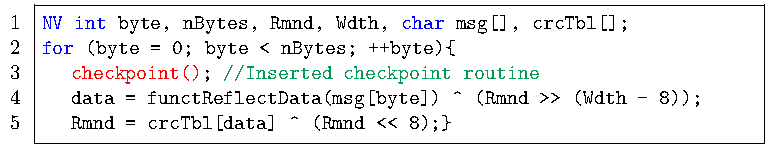
\includegraphics[width=\columnwidth]{figures/crc_example}\label{fig:crc_example}}\\
	\subfloat[Consecutive execution steps of the loop body in the snippet above: non-volatile checkpointing did not guarantee data consistency as data has been manipulated (line 10) with stale reminder (line 3)]{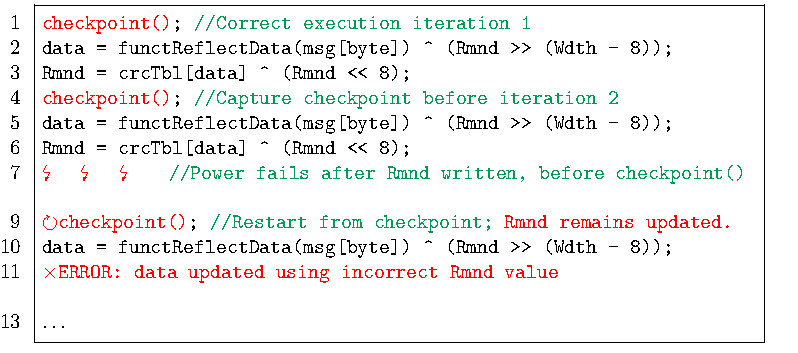
\includegraphics[width=\columnwidth]{figures/crc_example_war}\label{fig:crc_example_war}}
	\caption{Code example demonstrating effect of write after read on volatile memory checkpointing.}
	\label{fig:code_demo_incosistency}
\end{figure}


Data may become inconsistent if an attempt to execute some computation {\em
writes} to a non-volatile variable, then power fails, then a second attempt to
re-execute the same computation {\em reads} the value written in the first
attempt.  Figure~\ref{fig:code_demo_incosistency} illustrates how state can
become inconsistent in an intermittent execution using cyclic redundancy check
(CRC) code from MIBench~\cite{hicks_mibench2_2016}. The code computes CRC for
an $\texttt{nBytes}$ byte message $\texttt{msg}$ with remainder
$\texttt{Rmnd}$. Even with programmer defined checkpoints (i.e., line 3 in
Fig.~\ref{fig:crc_example}) of registers, stack, and non-volatile variables
(labeled \texttt{NV}), the code may compute  $\texttt{data}$ incorrectly.  The
code includes a write after read (WAR) hazard of variable $\texttt{Rmnd}$.  WAR
hazard is caused by consecutive write and read in-between two consecutive
checkpoints using $\texttt{checkpoint()}$ function: $\texttt{data}$ variable is
written \emph{before} (line 10 in Fig.~\ref{fig:crc_example_war})
$\texttt{Rmnd}$ is read (line 6 in Fig.~\ref{fig:crc_example_war}), or more
specifically---updated before a new execution loop. 

As the figure illustrates, checkpoint-based systems risk violating the
consistency of volatile and non-volatile memory~\cite{dino}. To maintain memory
consistency, versioning systems~\cite{dino,ratchet} {\em version} a subset of
non-volatile variables with the checkpointed execution context. Task-based
systems~\cite{chain,alpaca}, which we focus on this work and discuss in detail
next, ensure state is consistent by using programmer, compiler, and runtime
support.


\subsection{Task-based Intermittent Computing}
\TODO{This sequential / modular split seems pretty odd to me.  I think we can just talk about tasks in the sense of ratchet, alpaca, and chain.  Anything with static (programmer-written or compiler inserted) boundaries applies}
Intermittent execution models combatting WAR can be classified into: \emph{sequential execution model} (which historically formed a baseline for this stream of research) and \emph{modular execution model} (a potent alternative, on which we base the design decisions of \sys).
)

Under this model a program for intermittently-powered device is seen as a one idempotent operational region with one common context. Generally, the progress of the program is saved and updated by means of checkpointing, refer again to Section~\ref{sec:background_consistency}. Normally, the sequential model relies on a hardware assistant to measure the voltage level in the energy reservoir to place a checkpoint~\cite{mementos,mottola2017harvos,hibernus}. The benefit of this model is that it does not require code modification by a programmer. However it suffers from significant overhead (refer to experiment result in~\cite[Fig. 3]{chain}, where it is concluded that each checkpoint causes overhead). \todo{I use the word `checkpoint' for normal checkpoint and task boundary interchangeably---check if it does not cause confusion}{Brandon}


At the heart of this model is the concept of an \emph{idempotent task}. The idempotent task is a C language function that does not have arguments and does not return a value. This task uses a well defined interface to interact with the non-volatile memory. Therefore, it tolerates arbitrary number of power interrupts. This model, generally, produces less overhead~\cite{chain} and allows multiple applications to run on an intermittently-powered device by interleaving their tasks. However, it obviously requires code modification. For example, if an algorithm is written according to the continuous execution model it has to be split by a programmer into small tasks to run under the modular intermittent execution model.

Despite the benefit of the modular model certain limitations are still present that must be overcome and which inspired us to design \sys. Let us look at these problems in detail.

\begin{table}
	\centering
	\footnotesize
	\begin{tabular}{|c|c|c|c|}
		\hline
		{~} & CP & SZ & NV \\
		\hline\hline
		\!\!Mementos~\cite{mementos}\!\! & \!\!$N_2\leq N_1$\!\! & \!\!R + S\!\! & \!\!R + S\!\! \\
		\!\!DINO~\cite{dino}\!\! & $N_2$\!\! & \!\!R + W\!\! & \!\!R + W\!\! \\
		\!\!Chain~\cite{chain}, Alpaca~\cite{alpaca}\!\! & \!\!$N_2$\!\! & P\!\! & \!\!2W + P\!\!\\
		\!\!Ratchet~\cite{ratchet}, Clank~\cite{hicks_isca_2017}\!\! & $N_3\geq N_2\geq N_1$\!\! & \!\!R\!\! & R\!\!\\
		\hline 
	\end{tabular}
	\caption{Cost of various checkpointing methods; Symbols---R: register, S: stack, W: WAR-dependent variables, P: program counter, $N_1, N_2, N_3$: relative number of checkpoints for each method, CP: no. checkpoints, SZ: checkpoint size, NV: copy to non-volatile memory size.}
	\label{table:chechpoint_comparison}
\end{table}

\paragraph{Problem 1---Idempotent task is also costly}

The most important modular and intermittent models are compared in Table~\ref{table:chechpoint_comparison}\footnote{This table generalizes discussion from~\cite[Sec. 2.4]{alpaca}.}. Although we concluded that sequential execution model introduces a significant overhead, a modular approach also introduces certain execution penalty. Whatever the approach, the energy cost of a single checkpoint/idempotent task is $w\text{CP(SZ+NV)}$, where $w$ is the cost of a single word copy into a non-volatile memory. 

\begin{figure}
	\centering
	\subfloat[Energy cost of \emph{write} operation]{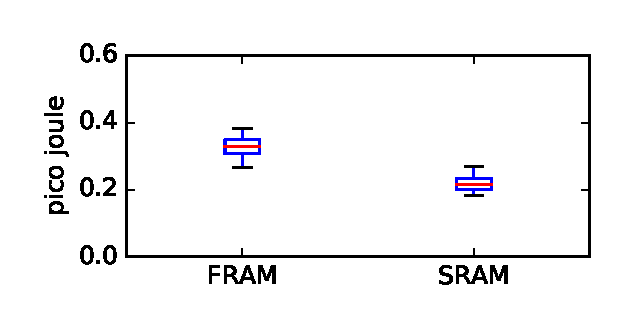
\includegraphics[width=0.49\columnwidth]{figures/fram_write.eps}}
	\subfloat[Energy cost of \emph{read} operation]{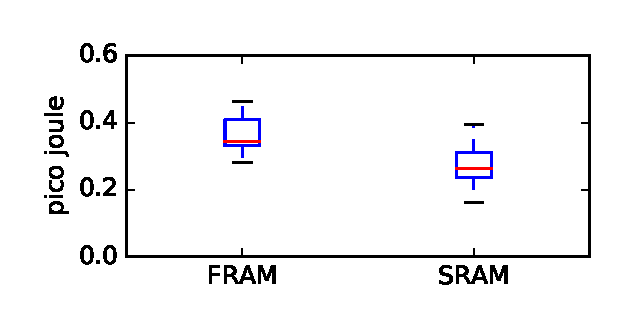
\includegraphics[width=0.49\columnwidth]{figures/fram_read.eps}}
	\caption{Energy cost of accessing volatile (SRAM)/non-volatile (FRAM) memory during write (left) and read (right) operation.}
	\label{fig:framEnergy}
\end{figure}

We have executed an experiment to measure the cost of read/write operations of $w$ to volatile and non-volatile memory. The result is given in Figure~\ref{fig:framEnergy}. Four applications were developed that \emph{access} the FRAM and SRAM of the MSP430FR5969 microcontroller~\cite{msp430datasheet}. The interference free debugger (EDB)~\cite{edb} is used as the energy measurement tool. The EDB probes the energy buffer before and after accessing the FRAM/SRAM 1600 times. This large number of FRAM access is used to increase the reliability of the results generated by the used measurement tool (e.g. reducing the effect of the quantization error). The energy buffer is charged, using the EDB, to $\approx$ 2.45\,V \textbf{only} at the beginning of the execution and of the programs. The write operations were performed by writing literal values, random numbers, to the memory. However, a read operation must be followed by a write operation. Therefore, we chose to write a read value to SRAM. Based on our measurements we conclude that a FRAM access equals $\frac{3}{2}$ SRAM access~\footnote{We remark that TI already mentions~\cite{ti_fram_faq} that FRAM write access is more energy expensive than SRAM write access. However, TI does not quantify this energy overhead.}. Therefore, reducing FRAM access is desirable when developing energy limited software solution---\emph{which is in sharp contrast to the main goal of all checkpoining solutions}.

The above result reassures the intuitive observation that a decrease of CP (Table~\ref{table:chechpoint_comparison}) decreases the energy cost associated with each state preservation method and reduces operation cost which in most simplistic terms is defined as $\mathcal{O}(\text{CP})+\mathcal{O}(\text{PL})$, where PL is the cost of program execution without checkpointing. On the other hand, this increases task/checkpoint re-execution time. The ideal solution is a runtime that \emph{adaptively} changes task size during runtime, which however exposes a second problem.

\paragraph{Problem 2---Modular execution models are not adaptive}

A modular intermittent execution model completely depends on a programmer's estimation which mostly results in a sub-optimal code division. Moreover, this model can only consider a single hardware configuration and it does not take environment variability into considerations. Each battery-less platform has different storage sizes, refer to Table~\ref{table:capacitor}, which causes different charge/discharge periods. This result in different execution times. In the worst case the size of the capacitor might be too small to execute one task written by the programmer. This calls for the ability of the modular execution runtimes to \textbf{merge} multiple small tasks into a larger one or \textbf{split} a large task into a set of small ones on the fly (post-compilation time). Unfortunately the following features prevent us to perform this task using existing runtimes~\cite{chain,alpaca}.

\begin{figure}
	\centering
	%\includegraphics[width=\columnwidth]{figures/Dynamic_chain_sequence_example}
	\caption{Dynamic task merging problem.\todo{Draw merging diagram}{Przemek/Amjad}}
	\label{fig:DynamicChainSeq}
\end{figure}

\begin{itemize}
	\item \textbf{Irreversible tasks transitions} According to both Chain~\cite{chain} and Alpaca~\cite{alpaca} programming models, each task calls the next one. The transition is done through functions calls and manually clearing the stack to prevent the stack overflow problem. This approach makes all the task transitions firm, preventing task merging.

	\item \textbf{Dependency on privatization} Alpaca~\cite{alpaca} extended Chain~\cite{chain} with a concept of privatization, i.e. it protects task-shared variables from WAR dependency problem \emph{within} the scope of a task. Therefore, if tasks are on-demand merged, the scope of these dependencies are changed and the static analysis to privatize these variables is not valid any more and the data consistency can not be preserved.

	\item \textbf{`All channels' requirement} Fig.~\ref{fig:DynamicChainSeq} shows that if the task control flow is a circular with no branches then task merging is possible. Moreover, all the intra-merged-tasks channel can be committed to SRAM instead of FRAM to save energy. However, this execution path is only a special one. If the general case (see again Fig.~\ref{fig:DynamicChainSeq}) is considered then leaving out the intra-merged-task channels might result in data inconsistency. Than is, if an application tries to access a merged task from the middle after a power interrupt then the input for that task is not ready, which result in an incorrect execution.
	
	\item \textbf{Lack of multi-versioning system} All known modular execution models define its own input for each task that is not shared with other tasks. This design decision makes the benefit of merging tasks of less importance since each task is interacting with its own variables. \todo{Rewrite this paragraph: still unclear}{Przemek}
\end{itemize}

\subsection{Main Idea: Tasks Coalescing}

To combat the above limitations we propose a new concept of \textbf{virtualization}: a modular execution model with softening a number of transitions, by keeping the state of the execution progress in the volatile memory, to construct a bigger \emph{virtual task} to reduce energy consumption. Ideally, the size of the virtual task should match the length of a continuous interval of the intermittent power supply for the best performance. Another form of virtualization can be achieved by reducing the number of non-volatile memory accesses. This can be done by having a temporary copy of a global variable in the volatile memory (similar to the caching principle) and a task interacts with it and updates it before writing back the most recent value to the non-volatile memory during the commit process.

\subsection{Assumption on the Type of Computing Hardware}
\label{sec:background_hardware}

Before proceeding further with the background we need to make certain assumptions about the underlying hardware. We assume that we operate on the microcontroller (more generally, computing hardware) equipped with a mix of volatile and non-volatile memory, such as FLASH, Ferroelectric RAM or Magnetoresistive RAM. We do not assume to rely on specific memory type (either volatile or non-volatile), in contrary to earlier works targeting non-volatile processors~\cite{su_date_2017,ratchet,quickrecall,nvp}. Actually, we will exploit the properties of both memory types to maximize performance metrics of the program being executed. We enable to I/O operations, however we do not enable the scheduling of operations (which \emph{nota bene} forms a foundation for a simple runtime). All in all, our hardware model follows in assumptions the two most relevant intermittently-powered execution environments~\cite{alpaca,chain}. \todo{Verify if this section is not out of place}{Brandon}

\subsection{Structuring a Task-based Intermittent Computing Program}

\todo{Please check this is the right way for this section: it reads as it should be in Section 3 describing \sys}{Brandon} Task is a programmer (or compiler) defined code that is executed based on consistent set of inputs, i.e. memory fetched from a specified memory location, producing a consistent output stored in a specified (the same or different) memory location. Syntactically, we can treat a task as a continuous sub-section of a large program encapsulated by (i) task specific keywords defining the beginning and the end of a task and (ii) message passing between tasks connected with each other.

\begin{figure}
	\centering
	%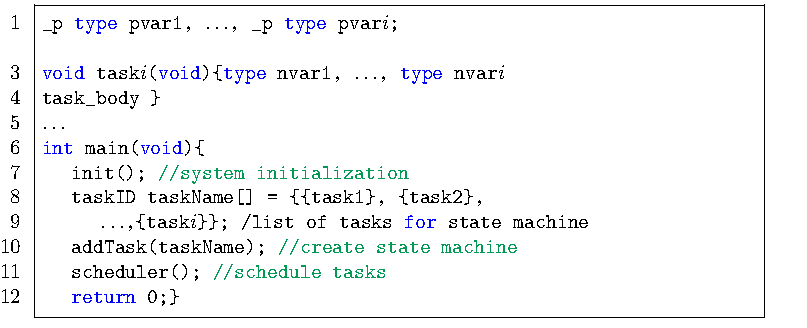
\includegraphics[width=\columnwidth]{figures/taskification_example}
	\caption{Task flow example executed by \sys.\todo{Draw an example task diagram}{Przemek}}
	\label{fig:task_flow_example}
\end{figure}

Let us look into how task-based programming is performed relying on an example provided in Fig.~\ref{fig:task_flow_example}. Each task is uniquely identified by a keyword. A separate part of code specifies a state machine than governs how tasks are connected with each other. This way a programmer specifies to which other task a current task needs to pass the result of its computation (and it can be either a new task or the task itself). Tasks are executed atomically. That is, task will be executed only once and will be considered as completed only when a task reaches a final instruction line informing a scheduler that a program is ready to enter into a new task.

Just like Chain~\cite{chain} and Alpaca~\cite{alpaca}, \sys does not support concurrent programming, multi-threading (multi-task sequence) and does not consider priorities and on-demand scheduling. These features are extremely important to consider but go beyond the scope of this work. A comparative description of \sys is given in Table~\ref{table:feature_comparison}. \todo{Decide if we need such table}{Brandon}

Important and a strong assumption about task-based programming for intermittently-powered systems is that an energy availability for the largest possible task execution must be guaranteed. Task is an atomic operation and must preserve execution order and memory manipulations. Task that follows such an assumption is equivalent to task being executed on a continuously-powered non-interrupted system. Whenever a task cannot fit into a single energy reservoir, it must be divided into tasks that will be executed within a single discharge cycle.

\begin{table}
	\centering
	\footnotesize
	\begin{tabular}{|c|c|c|c|}
		\hline
		{~} & Alpaca~\cite{alpaca} & Chain~\cite{chain} & This work \\
		\hline\hline
		Task connections & in-task & in-task & outside \\
		Task re-use & N & N & Y\\
		Memory model & globals & globals & globals\\
		Concurrency & N & N & N \\
		Task blocking & N & N & Y \\
		Energy-adaptive & N & N & Y \\
		\hline
	\end{tabular}
	\caption{Comparison of existing task-based execution models against \sys.}
	\label{table:feature_comparison}
\end{table}

\todo{Elaborate on the ``key challenge'' paragraphs near the end of the intro}{Przemek}

%We can write the problem of maximizing all task sizes formally as
%
%\begin{equation}
%\underset{i}{\arg\,\max} \sum_{i}m_i+t_i \text{~subject to~} \forall_i mi+t_i>e,
%\end{equation}
%
%where $e$ is the required minimum energy to perform a task, $i$ is the total number of tasks, $m_i$ and $t_i$ are the cost of task traversal (memory copying time of task variables) and time to complete one task, respectively.

%Two problems with fixed-size task in intermittent execution. (a) task underestimation: task executed at device with capacitor size $X$, will not execute at device with capacitor $X\gg Y$; (b) task overestimation: with stable energy source task tracking causes unnecessary overhead.

%\begin{figure}
%\centering
%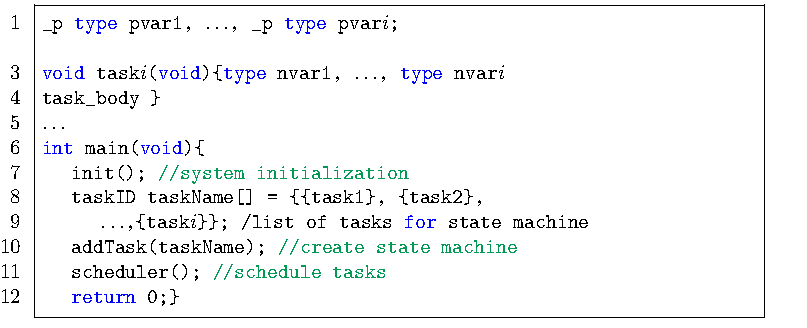
\includegraphics[width=\columnwidth]{figures/taskification_example}
%\caption{Program divided into tasks.}
%\label{fig:taskification_example}
%\end{figure}

%Other forms of intermittent platforms will share the same problem. One of them considers actuation platforms, which will be powered directly from energy harvesting sources~\cite{}. will share the energy storage with computing platform. However, power supply for actuators is order of magnitude larger than for computation. Therefore, although capacitor is large enough to perform computation alone, energy to power actuators takes precedence leaving not much space for computing.
